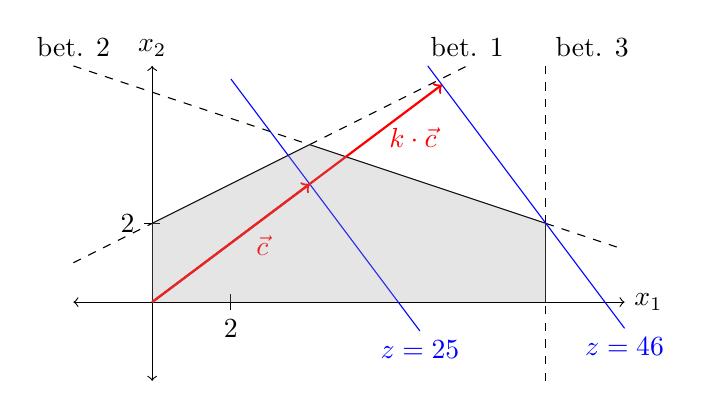
\begin{tikzpicture}
  %laver Grid. godt til når koordinater skal redigeres
  	%\draw[thin,gray!40] (-3,-1) grid (6,3); 
  %x-aksen
  	\draw[<->] (-1,0)--(6,0) node[right]{$x_1$}; 
  %y-aksen
  	\draw[<->] (0,-1)--(0,3) node[above]{$x_2$};
  	
  %akse-markeringer
  	%\node[left] (xakse) at (0,1) {2};
  	\draw[] (-0.1,1) -- (0.1,1) node[pos=0,left] {2};
  	\draw[] (1,-0.1) -- (1,0.1) node[pos=0,below] {2};
  	
  %ligning 1
	\draw[domain=-1:0,variable=\x,dashed] 	plot({\x},{0.5*\x+1});
	\draw[domain=0:2,variable=\x] 			plot({\x},{0.5*\x+1});
	\draw[domain=2:4,variable=\x,dashed] 	plot({\x},{0.5*\x+1}) node[above] {bet. 1};
	
  %ligning 2
  	\draw[domain=-1:2,variable=\x,dashed] 	plot({\x},{-(1/3)*\x+8/3}) node[above] at (-1,3) {bet. 2} ;
	\draw[domain=2:5,variable=\x] 			plot({\x},{-(1/3)*\x+8/3});
	\draw[domain=5:6,variable=\x,dashed] 	plot({\x},{-(1/3)*\x+8/3});
	

  %ligning 3
  	\draw[domain=-1:0,variable=\y,dashed] 	plot({5},{\y});
	\draw[domain=0:1,variable=\y] 			plot({5},{\y});
	\draw[domain=1:3,variable=\y,dashed] 	plot({5},{\y}) node[above right] {bet. 3};
	
  %niveaukurver
  	\draw[domain=3.5:6,variable=\x,blue] plot({\x},{-(4/3)*\x+23/3}) node[below] {$z=46$};
  	\draw[domain=1:3.4,variable=\x,blue] plot({\x},{-(4/3)*\x+25/6}) node[below] {$z=25$};
  	
  %c-vektor
  	\draw[->,thick,red] (0,0) -- node[pos=0.7,below=2] {$\vec{c}$} (2,1.5);
  	\draw[->,thick,red] (0,0) -- node[pos=0.9,below=4] {$k \cdot \vec{c}$} (3.68,2.76);

  %løsningsmængden skraveret
	\fill[gray!80,nearly transparent] (0,0) -- (0,1) -- (2,2) -- (5,1) --(5,0) --  cycle;
\end{tikzpicture}